\documentclass[]{article}

\usepackage[english]{babel}
\usepackage{graphicx}
\usepackage{booktabs}
\usepackage{float}
\usepackage{hyperref}

\title{Wind Prediction with LSTM}
\author{Juan Lao Tebar}

\begin{document}
	
\maketitle

\begin{abstract}
	
	TODO
	
\end{abstract}

\section{Introduction}

In this practice we extend the experiments performed in the previous ``Guided Laboratory of the RNN Topic''\footnote{https://upc-mai-dl.github.io/rnn-lab-guided/}, not only predicting more steps and trying more complex topologies, but also testing different ways of preparing the data to exploit the true power of LSTM networks, learning the inherent data relations over long intervals of time.

As explained in the guided laboratory, the data for this example is a subset of the NREL Wind Integration National Dataset (WIND) Toolkit\footnote{https://www.nrel.gov/grid/wind-toolkit.html}. The original set consists of meteorological information for more than 126,000 sites across the USA from 2007 to 2013, sampled every 5 minutes. However, for our purposes, we only take into account the data from one site sampled every 15 minutes.

In the guided laboratory we took into account only one variable---wind speed at 100m---and we predicted the value it takes in the following step. In contrast, in this practice we predict the following 6 steps including the rest of the variables: air density, temperature and air pressure.

The workflow of this practice consists in defining a baseline model---similar to the one proposed in the guided laboratory---and improving it in the following experiments, step by step.

In summary, these are the experiments we perform:

\begin{itemize}
	\item Effect of incrementing the number of hidden layers.
	\item Response of the model for different activation functions.
	\item Finding the appropriate window size.
	\item Regularizing an overfitted model applying dropout on \emph{all} activations---including LSTM gates.
	\item Avoiding explosive gradients with gradient clipping.
	\item Regularizing an overfitted model applying dropout \emph{only} on inter-layer connections.
	\item Presenting a new sequence-to-sequence model capable of learning from \emph{any-length} input samples.
\end{itemize}

The code related to this work is public and available at github\footnote{https://github.com/juanlao7/WIND-LSTM}.

\section{Experiments}

The original dataset consists of 245,472 measurements. In our process we use 122,736 of them for training---\~3.5 years---, 61,368 for validation and 61,368 for testing---\~1.75 years---. We decided to train and test our model in these large intervals of time due to the fact that weather depends on the time of the year and, since LSTM networks can learn data relations over long intervals of time, we may obtain better results when testing huge window sizes.

The loss of the model is measured with the mean squared error (MSE).

\subsection{Baseline}

Our first model is quite similar to the one proposed in the previous guided laboratory, as it consists of an LSTM layer of 512 units connected to a dense output layer of 24 units---6 predictions of 4 variables---, as it can be seen in figure \ref{f:model}. We use ReLU as the activation function of the LSTM activations, the logistic function in their recurrent step and, of course, a linear function for the output neurons.

\begin{figure}[H]
	\centering
	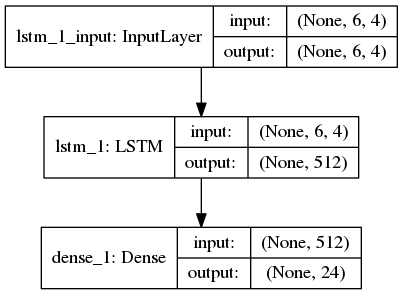
\includegraphics[width=0.5\textwidth]{model}
	\caption{Structure of the baseline model.}
	\label{f:model}
\end{figure}

% TODO: citar rmsprop
% TODO: buscar ref de recommended rmsprop

We train the model in batches of 1000 samples using the adaptive optimizer RMSprop---recommended for training recurrent neural networks---with a learning rate of 0.0001, $ \rho = 0.9 $, $ \varepsilon = 1 \cdot 10^{-8} $ and no learning rate decay. The samples are obtained by \emph{lagging} the original samples of the data set with their previous 6 steps and foreseeing the following 6.

In this practice we change the stopping criteria of the training process, as we remove the limit of epochs and we implement a stopper based on the validation loss: when we detect a minimum value, we stop the training after 30 epochs if it does not decrease.

With this configuration we obtain the results shown in table \ref{t:baseline}.

\begin{table}[H]
	\centering
	\begin{tabular}{@{}ccc@{}}
		\toprule
		Training loss & Validation loss & Test loss \\ \midrule
		0.02878       & 0.03151         & 0.03290   \\ \bottomrule
	\end{tabular}
	\caption{Results of the baseline model.}
	\label{t:baseline}
\end{table}

\subsection{Number of Layers}

% TODO ref esto

Feedforward neural networks with two hidden layers can represent an arbitrary decision boundary with arbitrary accuracy using rational activation functions, and approximate any smooth variable relation to any accuracy too.

In this experiment we compare our previous results with the ones obtained with models of two and three hidden LSTM layers of 512 units each.

Table \ref{t:layers} shows the results obtained and figure \ref{f:layers} shows the evolution of the training and validation loss in each case.

\begin{table}[H]
	\centering
	\begin{tabular}{@{}cccc@{}}
		\toprule
		& Training loss & Validation loss & Test loss \\ \midrule
		1 hidden layer  & 0.02878       & 0.03151         & 0.03290   \\
		2 hidden layers & 0.02771       & 0.03088         & 0.03257   \\
		3 hidden layers & 0.02830       & 0.03207         & 0.03327   \\ \bottomrule
	\end{tabular}
	\caption{TODO}
	\label{t:layers}
\end{table}

\begin{figure}[H]
	\centering
	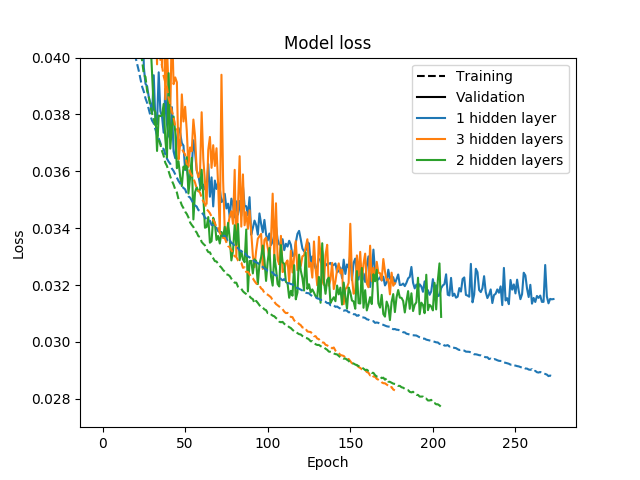
\includegraphics[width=0.5\textwidth]{layers}
	\caption{TODO}
	\label{f:layers}
\end{figure}

As expected, 2 hidden layers approximate better our data, while 3 hidden layers does not seem to have any effect. In the next experiments we use an architecture of 2 hidden LSTM layers.

\subsection{Activation Function}

Clevert, Unterthiner, \& Hochreiter, 2016 \cite{clevert2015fast} found that using ELU instead of ReLU not only speeds up the learning process in deep neural networks, but also leads to higher classification accuracies: ``In contrast to ReLUs, ELUs have negative values which allows them to push mean unit activations closer to zero like batch normalization but with lower computational complexity. Mean shifts toward zero speed up learning by bringing the normal gradient closer to the unit natural gradient because of a reduced bias shift effect''.

In this experiment we aim to reproduce similar results, testing different activation functions---softplus, logistic, hyperbolic tangent, ELU and ReLU---for the hidden LSTM layers of our model, but still using the logistic function for the recurrent step.

Table \ref{t:activation} shows the results obtained, while figure \ref{f:activation} shows the evolution of the training and validation loss in each case.

\begin{table}[H]
	\centering
	\begin{tabular}{@{}ccccc@{}}
		\toprule
		& Training loss & Validation loss & Test loss & Epochs \\ \midrule
		Softplus           & 0.02972       & 0.03352         & 0.03485   & 288    \\
		Logistic           & 0.02986       & 0.03217         & 0.03348   & 622    \\
		Hyperbolic tangent & 0.02864       & 0.03133         & 0.03289   & 172    \\
		ELU                & 0.02856       & 0.03143         & 0.03251   & 186    \\
		ReLU               & 0.02771       & 0.03088         & 0.03257   & 206    \\ \bottomrule
	\end{tabular}
	\caption{TODO}
	\label{activation}
\end{table}

\begin{figure}[H]
	\centering
	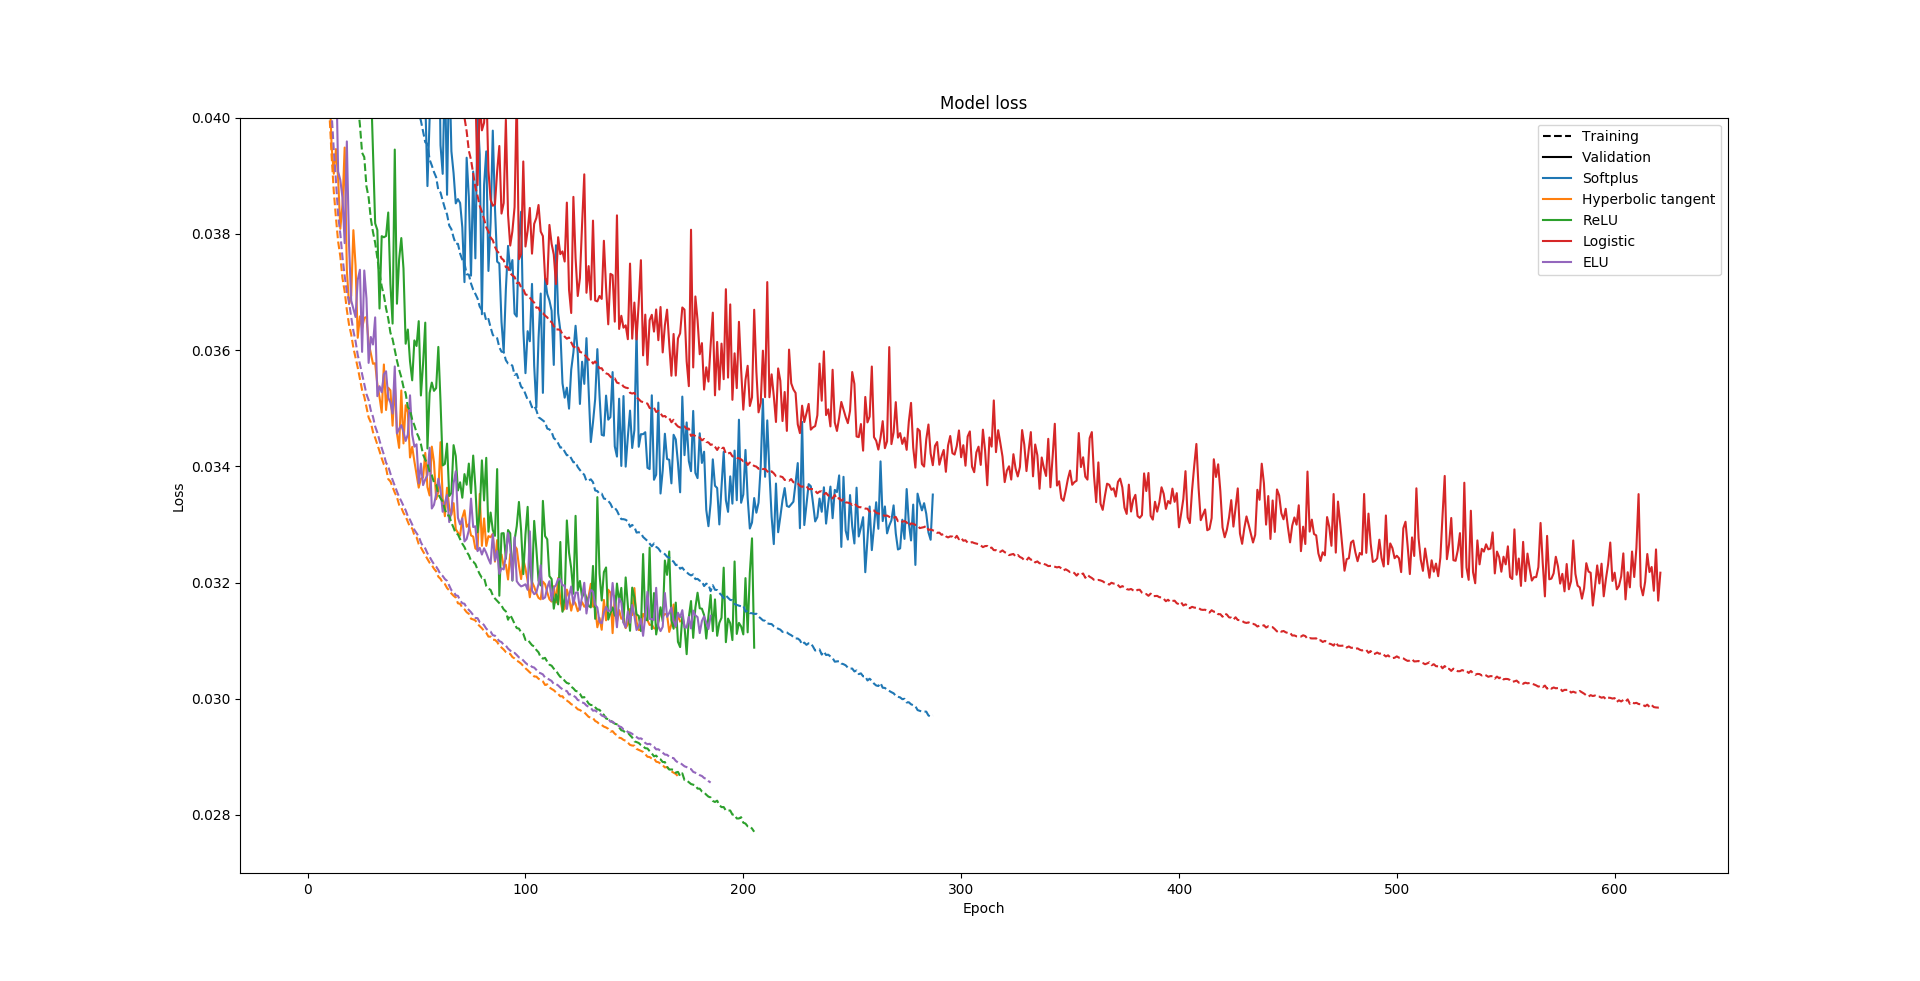
\includegraphics[width=\textwidth]{activation}
	\caption{TODO}
	\label{f:activation}
\end{figure}

As we can see, in our case ELUs and ReLUs are quite similar. We can see how ELUs take a slightly lower number of epochs to converge, with almost the same test loss then with ReLUs but higher training and validation losses.

In the following experiments we keep ReLU as the activation function for all the units of the hidden layers.

\subsection{Window Size}

Our data set is generated by going through the original samples with a window size of 12---6 measurements for the input, 6 for the output---. We must note that these measurements have been taken in intervals of 15 minutes, hence each input vector of the generated dataset comprises an interval of 75 minutes.

In this experiment we test different window sizes, in order to determine if larger time intervals provide useful information for our model to obtain a lower loss.

Table \ref{t:window} shows the results obtained, while figure \ref{f:window} shows the evolution of the training and validation loss in each case.

\begin{table}[H]
	\centering
	\begin{tabular}{@{}cccc@{}}
		\toprule
		& Training loss & Validation loss & Test loss \\ \midrule
		Input size of 1  & 0.03595       & 0.03743         & 0.03810   \\
		Input size of 6  & 0.02771       & 0.03088         & 0.03257   \\
		Input size of 12 & 0.02655       & 0.03190         & 0.03345   \\
		Input size of 24 & 0.02242       & 0.03655         & 0.03743   \\
		Input size of 48 & 0.01975       & 0.04247         & 0.04327   \\ \bottomrule
	\end{tabular}
	\caption{TODO}
	\label{window}
\end{table}

\begin{figure}[H]
	\centering
	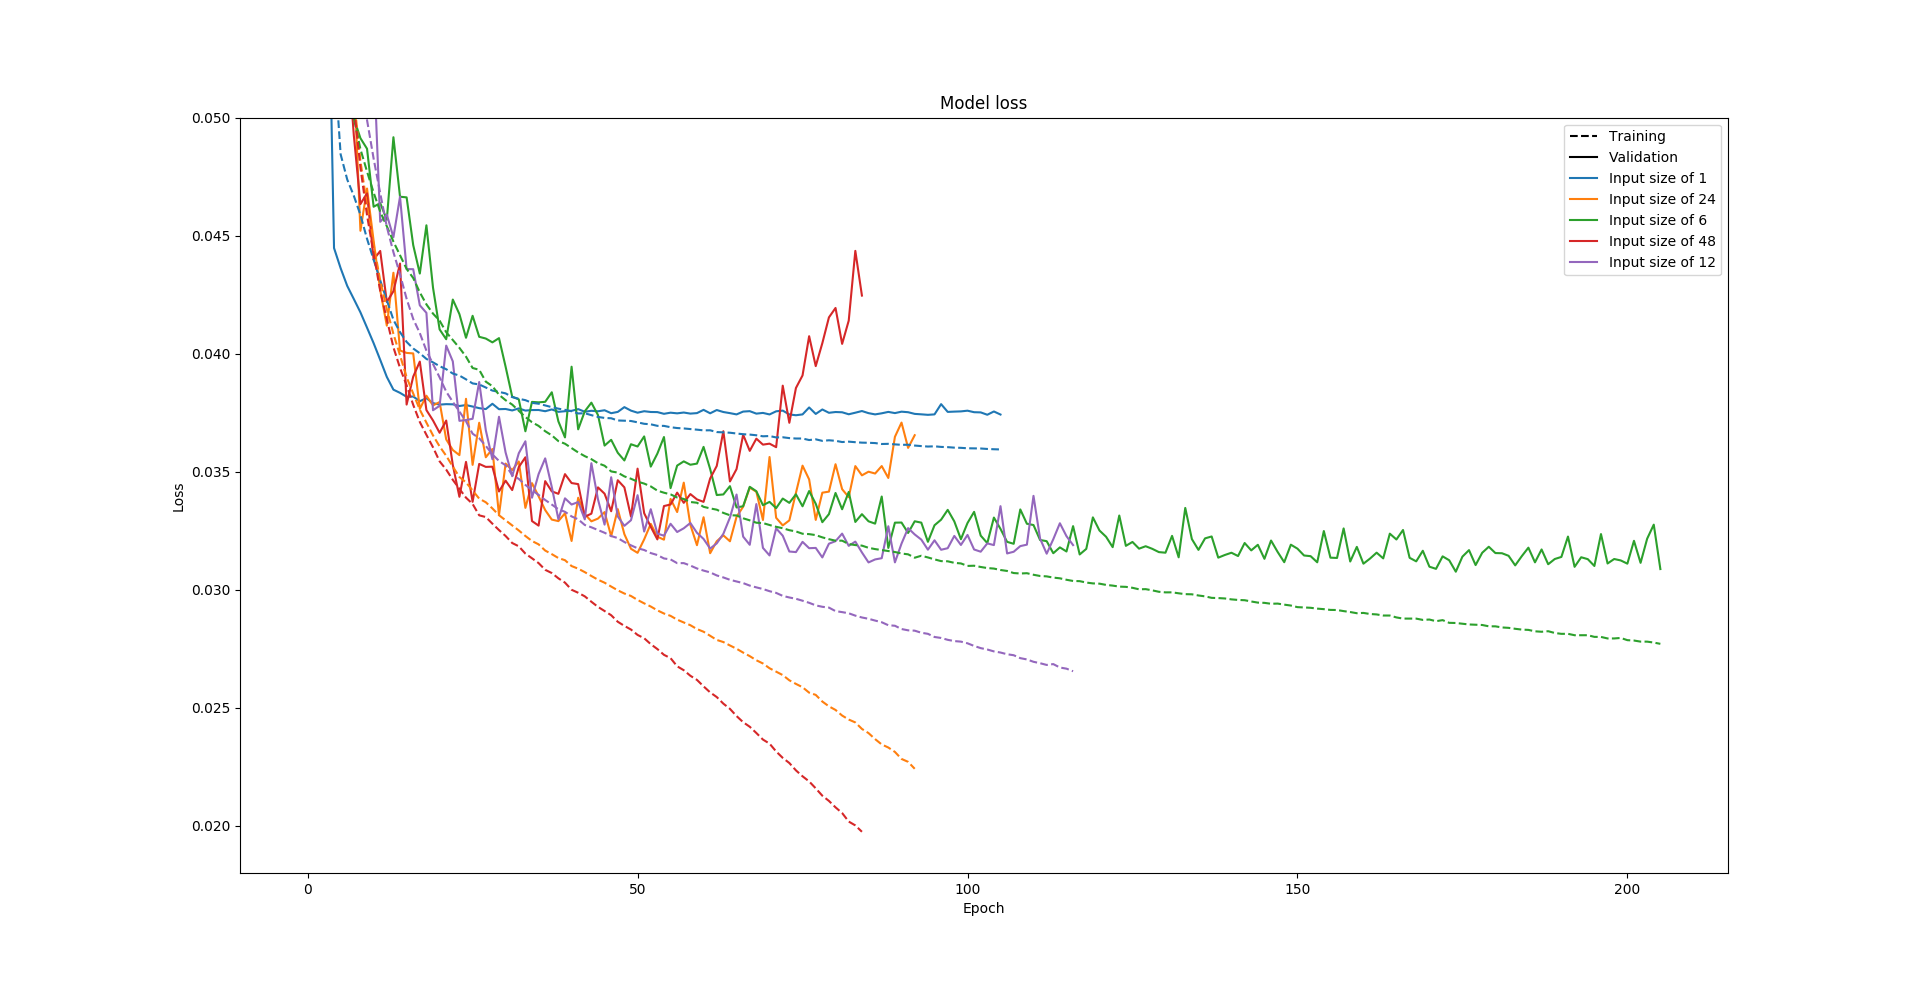
\includegraphics[width=\textwidth]{window}
	\caption{TODO}
	\label{f:window}
\end{figure}

In this experiment we test window sizes up to 48. When we test higher values, at some point the loss becomes $ +\inf $ and the training process fails. There can be several reasons behind this behaviour, but we suspect that it is due to a combination of using ELUs---which range is $ [-1, +\inf] $---and a high learning rate. However, when we try to use the logistic function we get worse results---as found in the previous experiment---and, when we decrease the learning rate, our experiments take too long to finish. For these reasons we decide to ignore bigger window sizes.

Regarding to the results, as we can see, bigger windows lead to lower training losses. In fact, our model overfits the data when we train it with sequences of 24 or 48 inputs, increasing the validation loss while decreasing the training error without any sign of convergence.

In the following experiments we continue working with the model with the best test loss---trained with sequences of 6 inputs---and the model with the best training loss---48 inputs.

\subsection{Dropout I}

Dropout is considered a simple and powerful regularization method. \cite{srivastava2014dropout} ``The key idea is to randomly drop units (along with their connections) from the neural network during training. This prevents units from co-adapting too much. During training, dropout samples from an exponential number of different ``thinned'' networks. At test time, it is easy to approximate the effect of averaging the predictions of all these thinned networks by simply using a single unthinned network that has smaller weights. This significantly reduces overfitting and gives major improvements over other regularization methods''.

In this experiment we apply different dropout values---25\%, 50\% and 75\%---in each LSTM layer, not only at the inter-layer connections but also at the recurrent step.

Table \ref{t:drop1} shows the results obtained, while figures \ref{f:drop11} and \ref{f:drop12} show the evolution of the training and validation loss in each case.

\begin{table}[H]
	\centering
	\begin{tabular}{@{}ccccc@{}}
		\toprule
		&      & Training loss             & Validation loss & Test loss       \\ \midrule
		Input size of 6  & 0\%  & 0.02771                   & 0.03088         & 0.03257         \\
		& 25\% & 0.14523                   & 0.09438         & 0.09005         \\
		& 50\% & 0.32983                   & 0.27392         & 0.25589         \\
		& 75\% & 0.63196                   & 0.55140         & 0.50822         \\
		\midrule
		Input size of 48 & 0\%  & 0.02231                   & 0.03864         & 0.04073         \\
		& 25\% & 40,982,524.64120          & 2,030,493.06455 & 2,327,123.48740 \\
		& 50\% & 0.29737                   & 0.26379         & 0.24811         \\
		& 75\% & 395,288,170,387,000.00000 & 191,750.24100   & 210,455.33092   \\ \bottomrule
	\end{tabular}
	\caption{TODO}
	\label{t:drop1}
\end{table}

\begin{figure}[H]
	\centering
	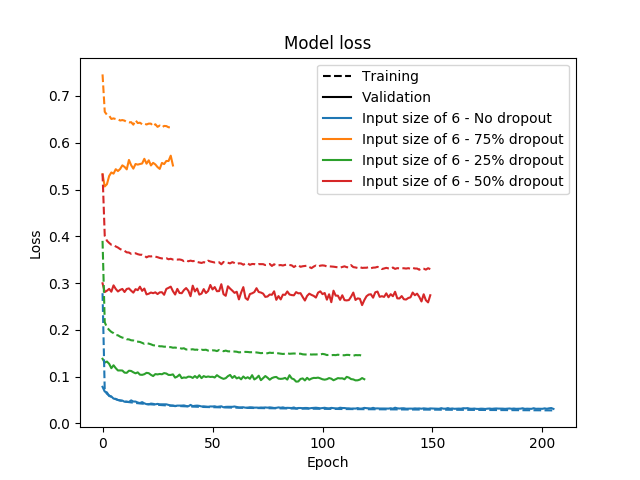
\includegraphics[width=0.5\textwidth]{drop11}
	\caption{TODO}
	\label{f:drop11}
\end{figure}

\begin{figure}[H]
	\centering
	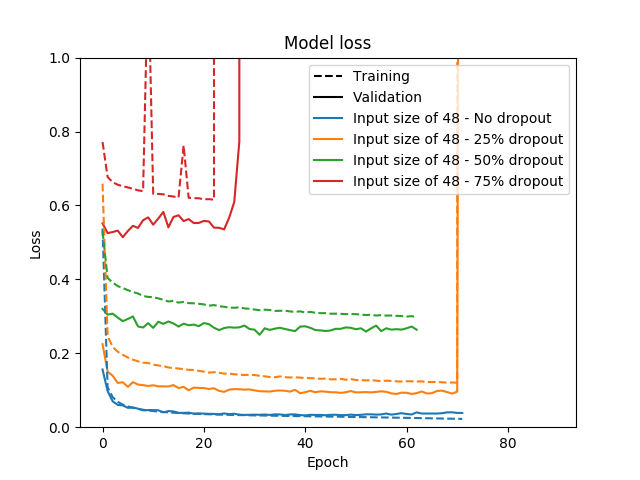
\includegraphics[width=0.5\textwidth]{drop12}
	\caption{TODO}
	\label{f:drop12}
\end{figure}

% TODO ref exploding gradients
As we can see, on input sizes of 48 samples, applying dropout cause a problem of exploding gradients, and our losses take very large values.

% TODO gradient clipping
Gradient clipping prevents gradients from exploding. As we can see in table \ref{t:drop2} and figure \ref{f:drop2}, when all parameter gradients are clipped to a maximum norm of 1 we can successfully train our models with dropout.

\begin{table}[H]
	\centering
	\begin{tabular}{@{}ccccc@{}}
		\toprule
		&      & Training loss & Validation loss & Test loss \\ \midrule
		Input size of 48 & 0\%  & 0.02248       & 0.03962         & 0.03925   \\
		& 25\% & 0.11694       & 0.09555         & 0.09036   \\
		& 50\% & 0.28648       & 0.27258         & 0.25334   \\
		& 75\% & 0.59369       & 0.51817         & 0.48055   \\ \bottomrule
	\end{tabular}
	\caption{My caption}
	\label{t:drop2}
\end{table}

\begin{figure}[H]
	\centering
	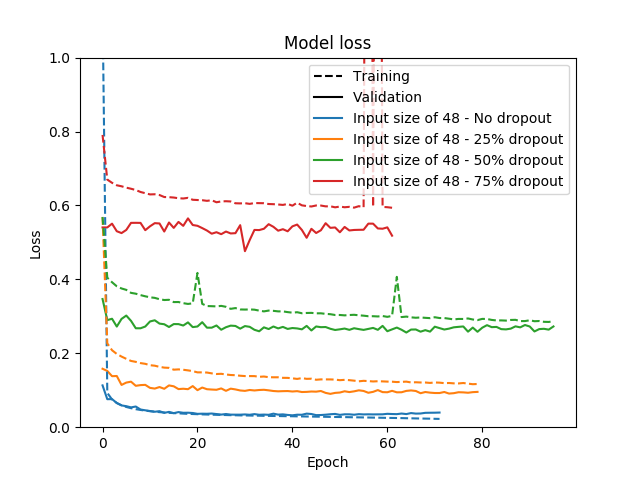
\includegraphics[width=0.5\textwidth]{drop2}
	\caption{TODO}
	\label{f:drop2}
\end{figure}

In our case, gradient clipping has demonstrated to be a good method for avoiding exploding gradients, hence we will conserve it in the following experiments. However, applying dropout at the inter-layer connections and at the recurrent step does not improve the performance of our model at all; on the contrary, it gets much worse.

\subsection{Dropout II}

Taking into account that LSTMs solve the vanishing gradient problem using an internal state controlled by gates, one may think that it may not be a good idea to apply dropout over those gates. It is possible that the bad results obtained in the previous experiment can be prevented just applying dropout at the inter-layer connections but not at the recurrent step.

In this experiment we apply different dropout values---25\%, 50\% and 75\%---after each LSTM layer.

Table \ref{t:drop3} shows the results obtained, while figures \ref{f:drop31} and \ref{f:drop32} show the evolution of the training and validation loss in each case.

\begin{table}[H]
	\centering
	\begin{tabular}{@{}ccccc@{}}
		\toprule
		&      & Training loss & Validation loss & Test loss \\ \midrule
		Input size of 6  & 0\%  & 0.02707       & 0.03102         & 0.03236   \\
		& 25\% & 0.03272       & 0.03107         & 0.03227   \\
		& 50\% & 0.04334       & 0.03215         & 0.03352   \\
		& 75\% & 0.06819       & 0.03617         & 0.03711   \\
		Input size of 48 & 0\%  & 0.02231       & 0.03864         & 0.04073   \\
		& 25\% & 0.03074       & 0.03451         & 0.03576   \\
		& 50\% & 0.03949       & 0.03425         & 0.03584   \\
		& 75\% & 0.06712       & 0.03815         & 0.03869   \\ \bottomrule
	\end{tabular}
	\caption{My caption}
	\label{my-label}
\end{table}

\begin{figure}[H]
	\centering
	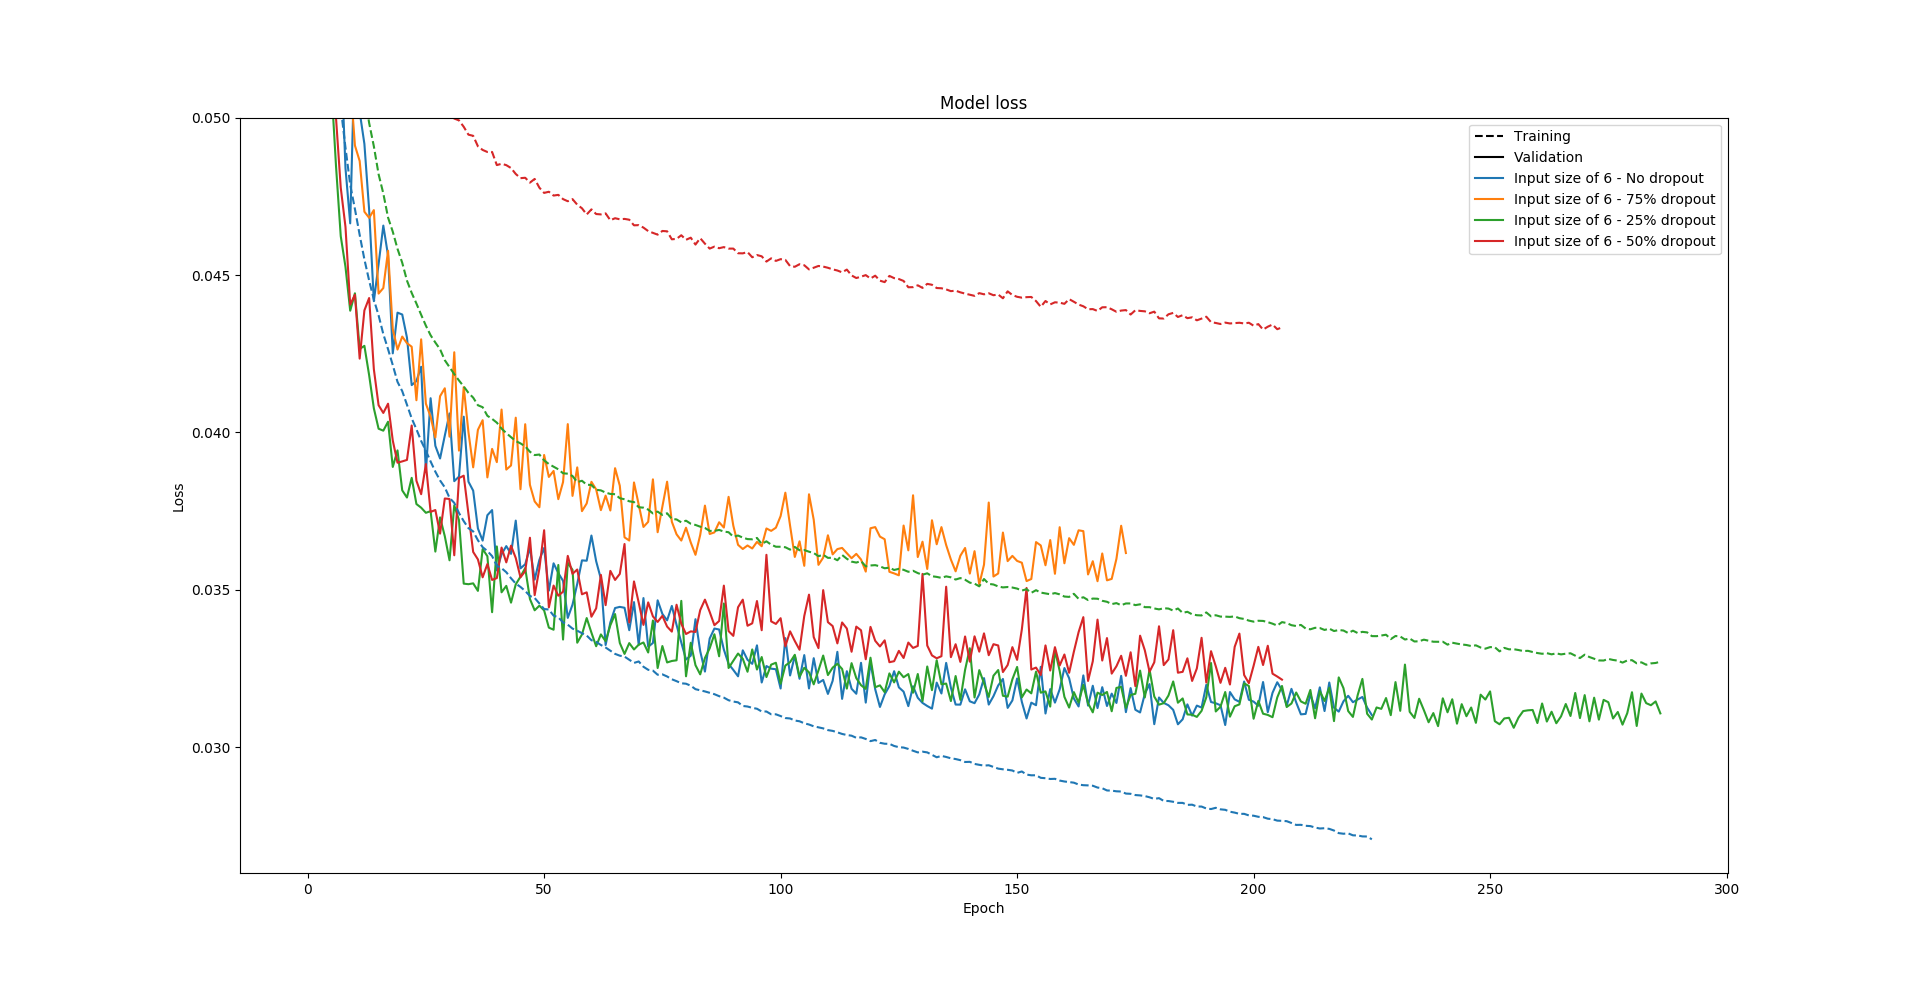
\includegraphics[width=\textwidth]{drop31}
	\caption{TODO}
	\label{f:drop31}
\end{figure}

\begin{figure}[H]
	\centering
	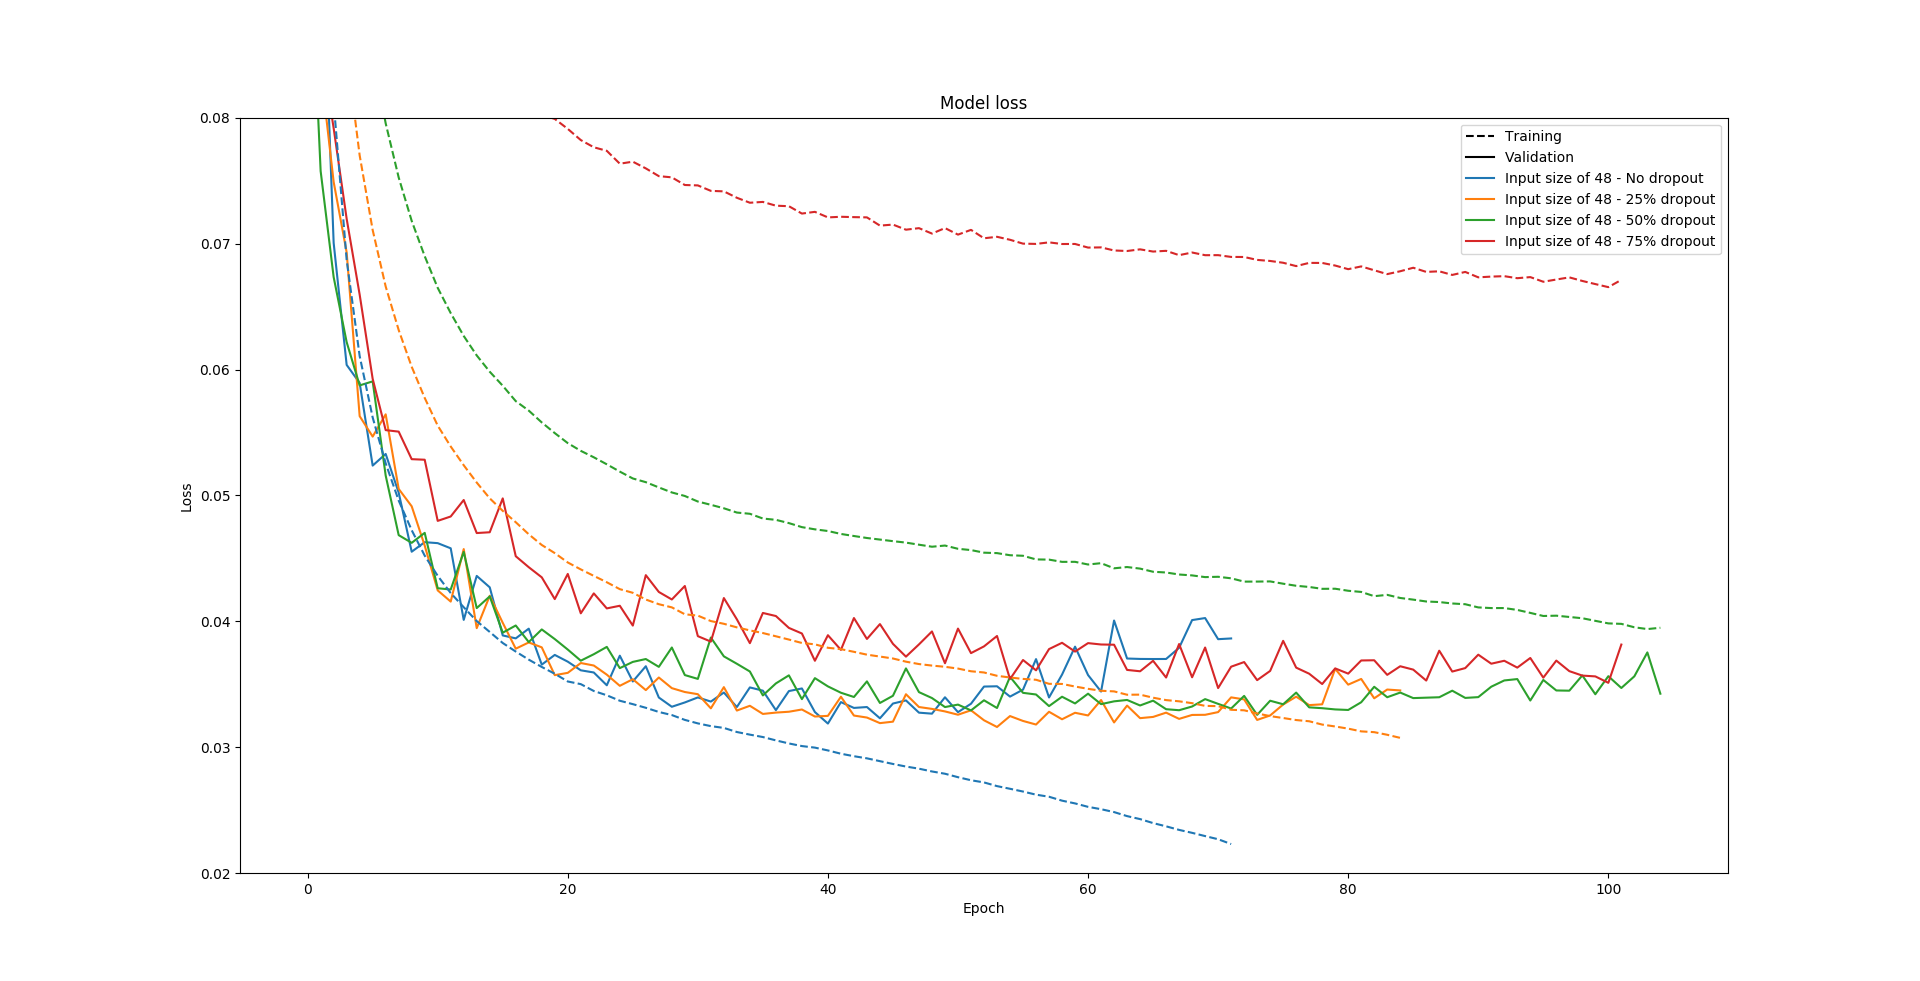
\includegraphics[width=\textwidth]{drop32}
	\caption{TODO}
	\label{f:drop32}
\end{figure}

As we can see, dropout does make any considerable improvement on the case in which the input size is 6---probably because that model was not overfitting the training data---; however, when the input size is 48, we can see how a dropout of 25\% successfully reduces the gap between training and validation losses, obtaining an overall lower test error.

In any case, the model with the bigger window size still has a worse performance than the model with an input size of 6. In the following experiment we only test this last model without dropout.

\subsection{Sequential Architecture}

LSTM networks can learn the inherent data relations between over intervals of time of \emph{any} length; however, in our current architecture, we are feeding the model with short subsequences generated with a small sliding window.

Why are we doing that? Can we train our LSTM with all our data set as a single sequence? If we do that, the LSTM network will learn whatever it finds relevant. It may happen that it finds data relations over large intervals of time, improving the overall performance of the system.

In our current architecture, if we try to process our data set with a huge window size, we find a physical problem.

When we process the data set, we go through $ N $ samples of $ V $ variables with a window size of $ W $, generating $ N - W $ vectors of $ V \cdot (W + 1) $ variables each. Since we train in batches of 1000, we are working with $ 1000 \cdot V \cdot (W + 1) $ variables simultaneously.

The memory used by this architecture directly depends on the size of sequences we use for training, making it not scalable for training with very large sequences. We would need large amounts of RAM to exploit the true power of LSTM networks.

To overcome this obstacle, in this experiment we present a new architecture with a model that gives a prediction for each input we feed to it (i.e. when we feed a sequence of $ N $ inputs, the model gives $ N $ outputs). This new architecture completely discards the sliding window process and directly feeds the original measurements to the model, targeting the next 6 measurements of the data set for each given input.

This new model uses an option defined by Keras framework in their LSTM layer implementation\footnote{https://keras.io/layers/recurrent/\#lstm}, the argument ``stateful'': ``Boolean (default False). If True, the last state for each sample at index $ i $ in a batch will be used as initial state for the sample of index $ i $ in the following batch''.

In this new architecture each element of the training sequences pertain to different batches and we feed them one by one, hence the RAM used by the training process is constant and it does not depend on the sequences size. In fact, now the required RAM only depends on the batch size we choose.

Our data is not compatible with this new training process and we must make a conversion first, since it is sequentially sorted by time. This conversion consists in reordering our data in such a way that, for a data set of $ N $ samples and a batch size of $ B $, samples from $ s_1 $ to $ s_{\frac{N}{B}} $ end up being the first elements of every batch, in sequential order; then samples from $ s_{\frac{N}{B}+1} $ to $ s_{\frac{N}{B}+\frac{N}{B}} $ end up being the second elements of every batch and so on. See figure \ref{f:explanation} for more details.

TODO EXPLANATION

As we can see, with this conversion we are training our model with $ B $ different sequences. Here we can decide how long we want our sequences: with a batch size of 1 we will train our model with a single sequence of 122,736 samples; with a batch size of 4 we will train our model 4 sequences of size 30,684.

In this experiment we leave the batch size as 1000---we train with input sequences of 122 samples---, in order to compare the results with the ones obtained in the previous experiments. We must leave the same batch size because it directly affects to the model’s generalization.

In this experiment we also clip all parameter gradients to a maximum norm of 0.000000001. Unfortunately we still suffer from exploding gradients, as it can be seen in figure \ref{f:architecture1}. This strict clipping slows the learning process; note that the gradients explode after after 2964 epochs---1 hour and 39 minutes---and the training loss is not even below 0.8. We could test lower clipping norms but then the training process would take an unfeasible amount of time to finish.

\begin{figure}[H]
	\centering
	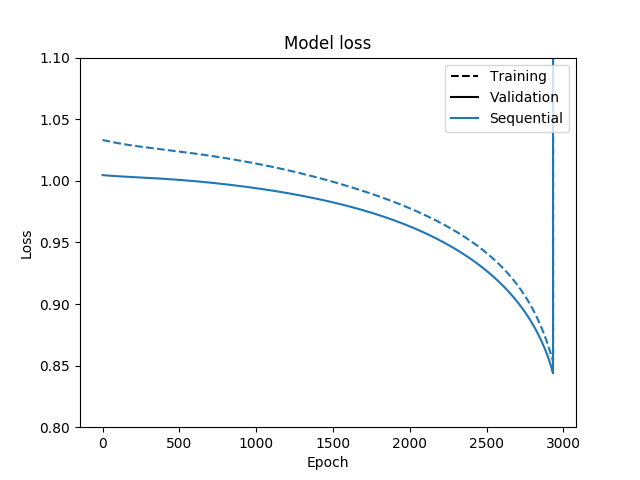
\includegraphics[width=0.5\textwidth]{architecture1}
	\caption{TODO}
	\label{f:architecture1}
\end{figure}

Our gradients are exploding due to the usage of ReLU, since its range is $ [0, +\inf] $. If we replace it with the hyperbolic tangent function---range $ [-1, 1] $---then we do not suffer from this problem.

Table \ref{t:architecture2} shows the results obtained, while figure \ref{f:architecture2} shows the evolution of the training and validation loss in each case.

\begin{table}[H]
	\centering
	\begin{tabular}{@{}cccc@{}}
		\toprule
		& Training loss & Validation loss & Test loss \\ \midrule
		Sequential      & 0.03556       & 0.04878         & 0.05231   \\
		Input size of 6 & 0.02707       & 0.03102         & 0.03236   \\ \bottomrule
	\end{tabular}
	\caption{My caption}
	\label{architecture2}
\end{table}

\begin{figure}[H]
	\centering
	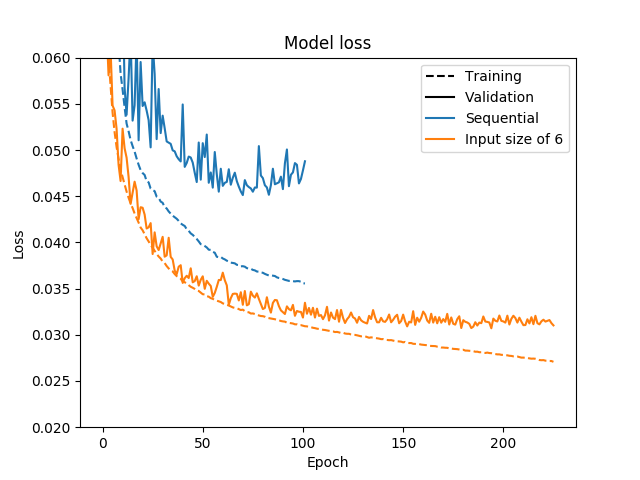
\includegraphics[width=0.5\textwidth]{architecture2}
	\caption{TODO}
	\label{f:architecture2}
\end{figure}

This new architecture may be useful for problems where the model needs to recall information far from the past (e.g., stock price prediction or paragraph understanding) but it does not offer any advantage over our previous architecture based on a sliding window. From the previous experiments, we already had the suspicion that all the relevant information for making a good prediction relies on the short past.

\section{Discussion of the Results}

\section{Conclusion and Future Work}

\end{document}
